\section{Results and Discussion}

\subsection{Geometric Properties}

To gain intuition for how they might affect patterns of tag connectivity, we began by surveying geometric properties of the tag matching metrics.

\begin{figure}
\begin{center}

\begin{subfigure}[b]{0.5\linewidth}
\centering
\includegraphics[width=\linewidth]{dimensionality-statistic}
\caption{
Dimensionality statistic
}
\label{fig:dimensionality_statistic}
\end{subfigure}%
\begin{subfigure}[b]{0.5\linewidth}
\centering
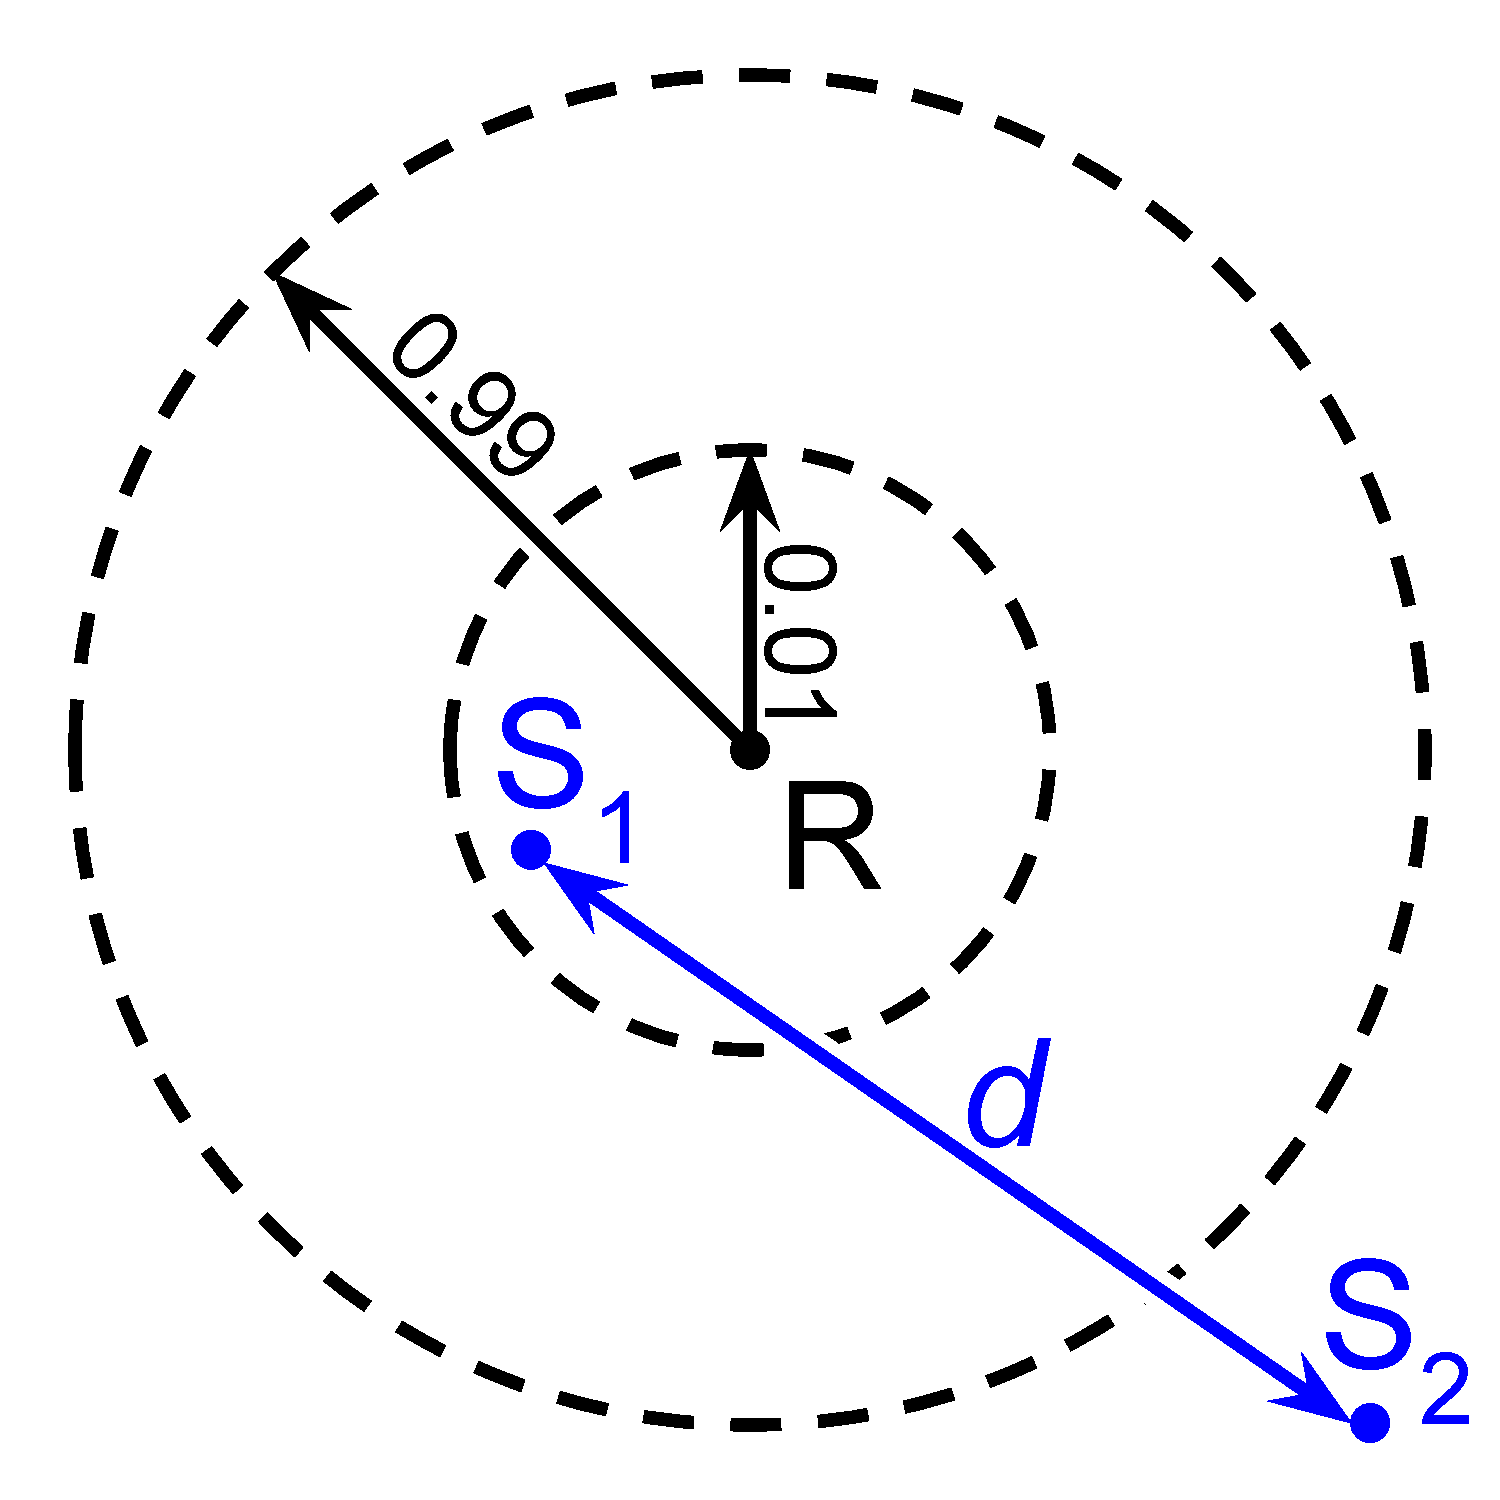
\includegraphics[width=\linewidth]{elasticity-statistic}
\caption{
Elsaticity statistic
}
\label{fig:elasticity_statistic}
\end{subfigure}

\caption{
A schematic depicting (A) the process used to generate the dimensionality statistic for each metric and (B) the process used to generate the elasticity statistic for each metric.
}
\label{fig:dimensionality_measure}

\end{center}
\end{figure}


\begin{figure*}
\begin{center}

\begin{minipage}{\linewidth}
\begin{subfigure}[b]{\linewidth}
\begin{minipage}{0.5\textwidth}
\begin{center}
\includegraphics[width=0.5\linewidth,trim=5cm 5cm 5cm 5cm, clip]{img/dimensionality-statistic}
\end{center}
\end{minipage}%
\begin{minipage}{0.5\textwidth}
\caption{
Sampling process used to measure similarity constraint.
First, a constraining tag $R$ was randomly sampled.
Then, tags were randomly drawn until two tags $S_1$ and $S_2$ with distance to $R$ less than 0.01 were obtained.
Finally, similarity constraint was measured as the distance $d$ between $S_1$ and $S_2$.
}
\label{fig:dimensionality_measure}
\end{minipage}
\end{subfigure}
\end{minipage}
\begin{subfigure}[b]{\linewidth}
\begin{minipage}{0.6\linewidth}
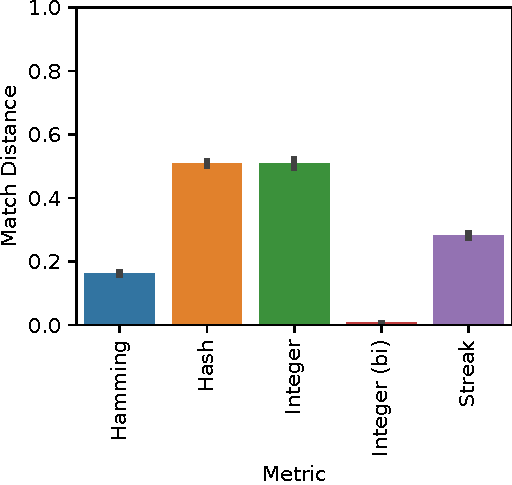
\includegraphics[width=\linewidth]{img/sphere/bitweight=0dot5+seed=1+title=dimensionality_barplot+_data_hathash_hash=c0f6c5cf854ff253+_script_fullcat_hash=03ce1e318a24a109+ext=}
\end{minipage}
\begin{minipage}{0.35\linewidth}
\caption{
Mean similarity constraint.
Error bars represent 95\% confidence intervals.
}
\label{fig:sphere_barplot}
\end{minipage}
\end{subfigure}
\begin{minipage}{\linewidth}
\begin{subfigure}[b]{\linewidth}
\centering
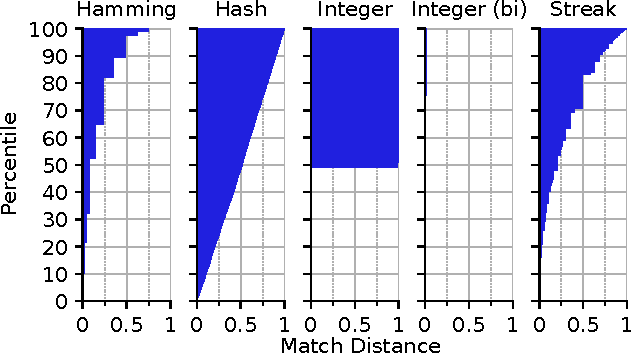
\includegraphics[width=\linewidth]{img/sphere/bitweight=0dot5+seed=1+title=dimensionality_distnplot+_data_hathash_hash=c0f6c5cf854ff253+_script_fullcat_hash=bea2a31376bf6bd0+ext=}
\begin{minipage}{0.8\textwidth}
\caption{
Distributions of sampled similarity constraint values.
Each visualization arranges individually sampled observations (thin horizontal bars) vertically in descending order.
The $y$ axis can be interpreted as ranging form the \nth{0} percentile of outcomes (bottom) to \nth{100} percentile (top) with horizontal bar width showing similarity constraint at a certain percentile.
}
\label{fig:sphere_distnplot}
\end{minipage}
\end{subfigure}
\end{minipage}

\caption{
Similarity constraint of tag-matching metrics.
Figure \ref{fig:dimensionality_measure} summarizes the sampling process used to measure similarity constraint.
Figures \ref{fig:sphere_barplot} and \ref{fig:sphere_distnplot} compare distributions of similarity constraint across metrics.
}
\label{fig:sphere}

\end{center}
\end{figure*}


To gain a sense of the dimensionality (in a loose sense) of the different tag-matching metrics, we sampled the distribution of distances between within a 0.01 match distance radius of an arbitrary target.
We used 5000 samples.
Figure \ref{fig:dimensionality_measure}a provides a cartoon summary of this process.

In a euclidean space, this would correspond to the average distance between points uniformly sampled from inside a ball (in two dimensions, a circle, and in three dimensions, a sphere).
This statistic asymptotically increases with dimensionality (TODO show this with mathematica, also try to calculate asymptote).
In one dimension, this value approximates to 0.00666667 \citep{dunbar1997average}.
In two dimensions, 0.00905415 \citep{dunbar1997average}.
In 32 dimensions, 0.0136618 \citep{dunbar1997average}.

We calculated this statistic as 0.0068 for the bidirectional integer metric, in line with expectations.
As you can see in Figure \ref{fig:sphere_distnplot}, the distances are all bounded by the diameter of 0.02.

However, other metrics had much higher values.
For the Spector Integer metric, we approximated this value as 0.494225945397328.
This is an artifact of the asymmetry where if you have two very similar numbers, half will be in ascending order resulting in a match distance close to 0 and half will be in descending order, resulting in a wraparound search and a match distance close to 1.
You can very clearly see these two outcomes in \ref{fig:sphere_distnplot}.
Averaging this out yields 0.5.

The uniformified hamming had a mean distance of 0.1724647213464.
In our sample, we observed distances as high as 0.756315.
To check our intuition, we calculated this statistic for the raw hamming metric.
For numerical reasons, we raised the radius of our sampling sphere to 0.25 (e.g., with a radius of 0.01, the only result between is a perfect match and with lower radii the hits become so rare as they become difficult to sample efficiently)
in 32 dimensional euclidean space, we expect the mean distance between sampled points to be 0.341545.
In the non-uniformified hamming metric we calculate this statistic as 0.33120625.
The distortion of the uniformification is clearly affecting this statistic with respect to the hamming metric.

We calculated an even higher value of 0.27255493763596844 for the ball sampling statistic with the streak metric.
We calculated distances as high as 0.999346.

For the hash metric, we calculated the ball sampling statistic as 0.17135186630635799.
A well-behaved hash should, given any set of operands, yield hash results uniformly distributed over the range.
However, this doesn't appear to be the case with \texttt{combine\_hash} for tags sampled within a ball.
As can be seen within \ref{fig:sphere_distnplot}, the majority of hash outcomes were distributed towards all zero bitstrings and or, in smaller proportion, to all one bitstrings.
We believe this to be an artifact of the particular hash methodology employed.

\begin{figure}
\begin{center}

\begin{subfigure}[b]{\columnwidth}
\centering
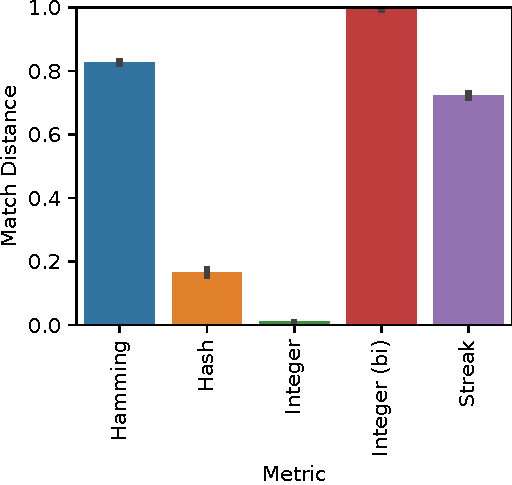
\includegraphics[width=\columnwidth]{{{sphere_reverse/bitweight=0.5+seed=1+title=dimensionality_barplot+_data_hathash_hash=7eaa832497d2f3cb+_script_fullcat_hash=03ce1e318a24a109+ext=}}}
\caption{
TODO
}
\label{fig:sphere_reverse_distnplot}
\end{subfigure}


\begin{subfigure}[b]{\columnwidth}
\centering
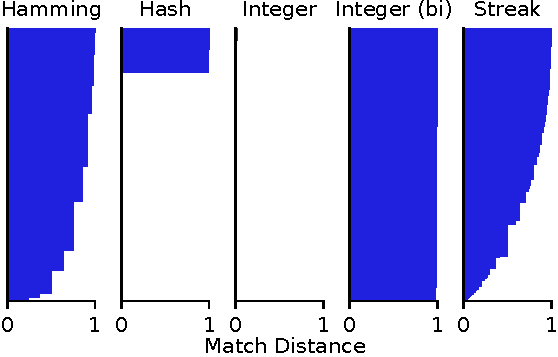
\includegraphics[width=\columnwidth]{{{sphere_reverse/bitweight=0.5+seed=1+title=dimensionality_distnplot+_data_hathash_hash=7eaa832497d2f3cb+_script_fullcat_hash=03ce1e318a24a109+ext=}}}
\caption{
TODO
}
\label{fig:sphere_reverse_barplot}
\end{subfigure}

\caption{
TODO
}
\label{fig:sphere_reverse}

\end{center}
\end{figure}


We tested the elasticity of the tag-matching metrics using a similar measure.
To gain a sense of the dimensionality (in a loose sense) of the different tag-matching metrics, we sampled the distribution of distances between a tag sampled from within a 0.01 match distance radius of an arbitrary target and a tag sampled from outside a 0.99 match distance radius of the arbitrary target.
We used 5000 samples.
Figure \ref{fig:dimensionality_measure}b provides a cartoon summary of this process.

We found that the bidirectional integer metric was highly inelastic: the smallest distance between the sampled tags was 0.980201.
The mean distance between sampled tags was 0.9932740098.
The Spector integer metric exhibited similarly uniform outcomes, except the distribution was strongly pegged to 0 because of the metric's asymmetry.
The mean statistic was 0.00998706165234.

The hamming metric exhibited greater elasticity: we observed distances between the sampled tags as low as 0.243549.
The mean distance between sampled tags was 0.8266405957999999.

The hamming metric exhibited the greatest elasticity: we observed distances between the sampled tags as low as 0.0011994999999999998.
With this metric, a tag can have a strong attractive interaction with a second tag that a third tag it interacts attractively strongly with has a strong repulsive attraction with.
The mean distance between sampled tags was 0.723582315152.

The hash metric exhibited the same poorly behaved non-uniform distribution as before, with a mean distance of 0.16510482108441799.

\begin{figure}
\begin{center}

\begin{minipage}{\linewidth}
\begin{subfigure}[b]{\linewidth}
\begin{minipage}{0.5\textwidth}
\begin{center}
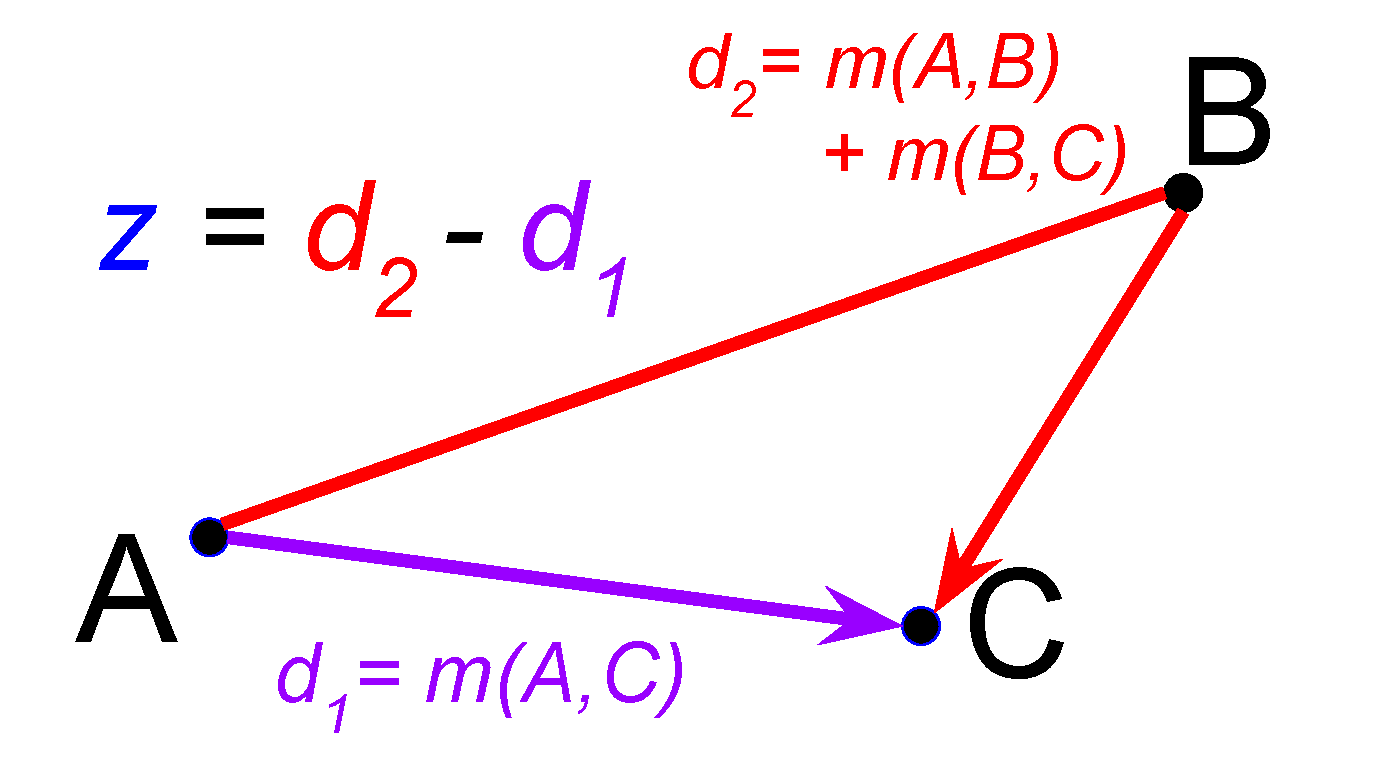
\includegraphics[width=\linewidth,trim=2cm 5cm 2cm 5cm, clip]{detour-difference}
\end{center}
\end{minipage}%
\begin{minipage}{0.5\textwidth}
\caption{
Sampling process used to evaluate detour difference, $z$.
} \label{fig:detour_difference_cartoon}
\end{minipage}
\end{subfigure}
\end{minipage}

\begin{minipage}{\linewidth}
\begin{subfigure}[b]{\linewidth}
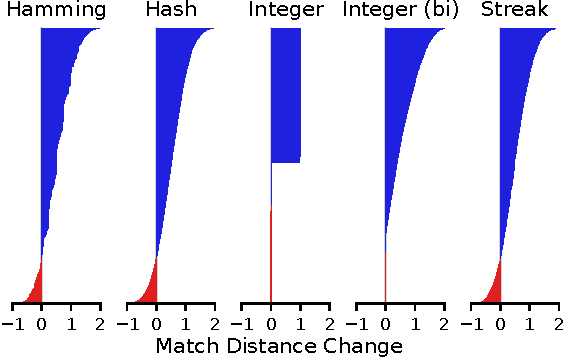
\includegraphics[width=\linewidth]{detour_difference/bitweight=0dot5+seed=1+title=low-triplet-analysis+_data_hathash_hash=6b0749ef97a58721+_script_fullcat_hash=297c4fe09078e17b+ext=}
\caption{
Distributions of detour distance difference for triplets of randomly sampled tags.
Each bar sliver represents an independently sampled observation.
A positive value (colored blue) indicates that total distance increased with the addition of an intermediate stop.
A value of exactly 0 indicates an intermediate stop had no effect on total distance.
A negative value (colored red) indicates violation of the triangle inequality: taking an intermediate stop reduced the total distance travelled.
} \label{fig:detour_difference_distribution}

\end{subfigure}
\end{minipage}

\caption{
Detour difference of tag-matching metrics.
}
\label{fig:detour_difference}

\end{center}
\end{figure}


To get a sense of the regularity, in a looses sense, of each space we uniformly sampled triplets of points $A$, $B$, and $C$.
Then, for each metric $m$ we calculated the statistic $m(A, B) + m(B, C) - m(A, C)$.
If the triangle inequality is respected this statistic should be greater than or equal to zero.
Figure \ref{fig:detour_difference} plots the distribution of this statistic for each metric.
The hamming and streak metrics show evidence of ``shortcuts'' that violate the triangle inequality.
It should be noted that the raw hamming metric does respect the triangle inequality.

\subsection{Variational Properties}

\begin{figure}
\begin{center}

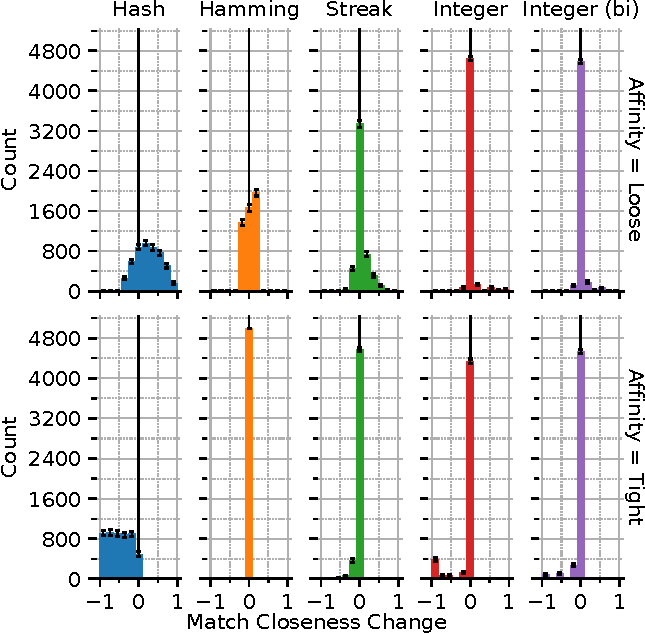
\includegraphics[width=\columnwidth]{img/mutational_step/bitweight=0dot5+seed=1+title=low-mutational-step+viz=hist+_data_hathash_hash=95a57768de56995a+_script_fullcat_hash=aa068ad24b386169+ext=}
\caption{
Distributions of mutation effects on match distance for loosely matched (pre-mutation match distance $> 0.5$) and tightly matched (pre-mutation match distance $< 0.01$) tag pairs.
Note that match closeness change (rather than mast distance change) is plotted so that better-matching mutational outcomes fall to the right and worse-matching mutational outcomes fall to the left.
Error bars are 95\% confidence intervals calculated using the Wilson score method with continuity correction \citep{newcombe1998two}.
Supplementary Figure \ref{fig:mutational_step_supp} shows the cumulative distribution of all sampled match distance changes for each metric.
}
\label{fig:mutational_step}

\end{center}
\end{figure}


We began by analyzing the distribution of single-bit mutations on match scores under the different metrics.
Figure \ref{fig:mutational_step} provides this analysis for two categories of tag pairs: loosely matched and tightly matched.
To generate the loosely matched distribution we unifomormly selected from tag pairs with a match distance > 0.5, measured their match distance, applied a one-bit mutation to the second tag, and then measured their match distance again.
To generate the tightly matched distribution we picked a target tag.
Then, we uniformly sampled a second tag with a match distance < 0.01.
We measured their match distance, applied a one-bit mutation to the second tag, and then measured their match distance again.
We sampled 5000 measurements for each affinity and each metric.

For both tight and loose affinities, although the integer metrics exhibited no perfectly neutral mutational outcomes most mutations cause very small change in the match score.
These are mutations to the least-significant bits of the bitstring.
A small fraction of mutations under these metrics, affecting the more-significant bits of the bitstring, have a stronger effect.
The integer metrics, along with the hash metric, exhibit the strongest one-step decoupling mutations under tight affinity.
The Spector integer metric, in particular, due to its asymmetrical wraparound-search inducing effect, exhibits more frequent strong decoupling mutations than the bidirectional integer metric.

The streak metric alone exhibits a portion of perfectly neutral outcomes under mutation.
The streak metric exhibits a greater fraction of mutational outcomes of non-trivial magnitude than the integer metrics with loose affinity.
Under tight affinity, the streak metric exhibits some one step strong-decoupling mutations but less intensely than the integer metrics.

The hamming metric exhibits more uniformity in the magnitudes of mutational effects than other metrics under both tight and loose affinities.
The hamming metric exhibits no perfectly neutral mutational outcomes.
(Without uniformification, all hamming metric mutations are of excactly the same magnitude with respect to match score).

The hash metric exhibits the greatest fraction of non-trivial mutational effects and exhibits some mutational intensities as extreme as the integer metrics.

\begin{figure*}
\begin{center}

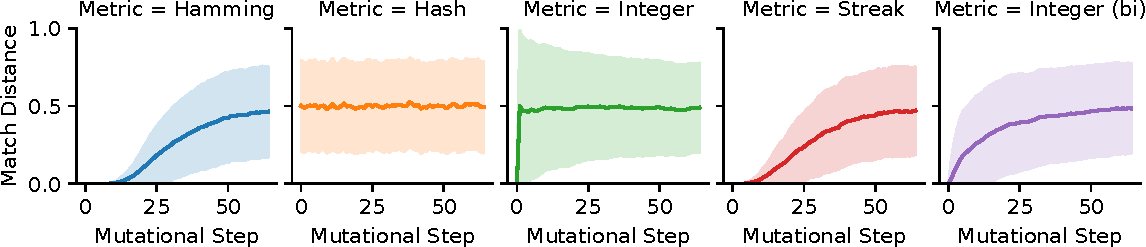
\includegraphics[width=\textwidth]{{{mutational_walk/bitweight=0.5+seed=1+title=mutational_walk_lineplot+_data_hathash_hash=ff15c8831d4f9288+_script_fullcat_hash=c872df869f05035a+ext=}}}
\caption{
TODO
}
\label{fig:mutational_walk_lineplot}

\end{center}
\end{figure*}

\begin{figure}
\begin{center}

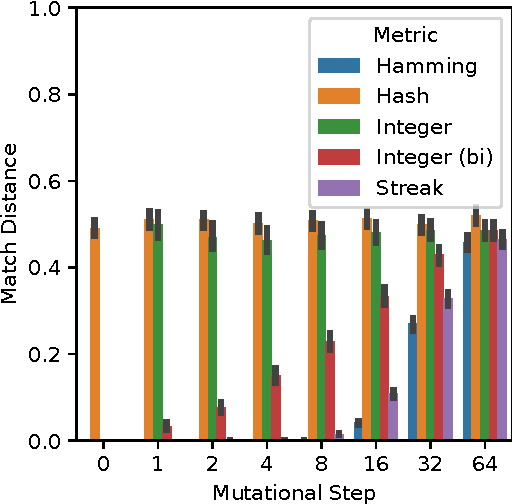
\includegraphics[width=\columnwidth]{{{mutational_walk/bitweight=0.5+seed=1+title=mutational_walk_barplot+_data_hathash_hash=8bf152d87daa9cb7+_script_fullcat_hash=982405ca713eba73+ext=}}}
\caption{
Snapshots of match distance at exponentially increasing steps from identical tags.
Error bars represent 95\% confidence intervals.
}
\label{fig:mutational_walk_barplot}

\end{center}
\end{figure}


Next, we performed mutational walks under each metric.
We began with two randomly chosen equivalent tags (mutation step zero) then applied randomly chosen one-step mutations (with the possibility of back mutation allowed) 65 times to the second tag.
We measured match distance between the two tags at each mutational step.
We performed 1000 independent mutational walks from different starting equivalent tags.

Figure \ref{fig:mutational_walk_lineplot} continuously depicts the distribution of match distances on mutational walks, with shaded areas indicating standard deviation, under different metrics.
Figure \ref{fig:mutational_walk_barplot} compares match distances at exponentially increasing steps.
Error bars indicate 95\% confidence intervals.

For the hash metric, where equivalent tags don't necessarily have low match distance, the mutational walk wanders around loose affinity.

The Spector Integer metric, where half of mutational steps wrap back around to 1.0 distance, immediately spikes up to an average match distance of 0.5.
The variance decreases with mutational steps as the distribution moves away from bias towards distances of 0 and 1.

The bidirectional integer metric experiences a greater immediate jump in variance and significantly greater mean match distance as rare mutations affecting significant bits take place (non-overlapping 95\% CI).

The
Intrestingly, contrary to as was claimed in \citep{downing2015intelligence}, the uniformified streak metric's match score under mutation actually grows significantly faster than the hamming metric's match score  (non-overlapping 95\% CI).

Because the are uniformified, the distributions all devolve to having an equivalent mean and variance.

\subsection{Target Graph Matching Evolutionary Experiment}

\begin{minipage}{\linewidth}
\begin{center}

\begin{minipage}{\linewidth}
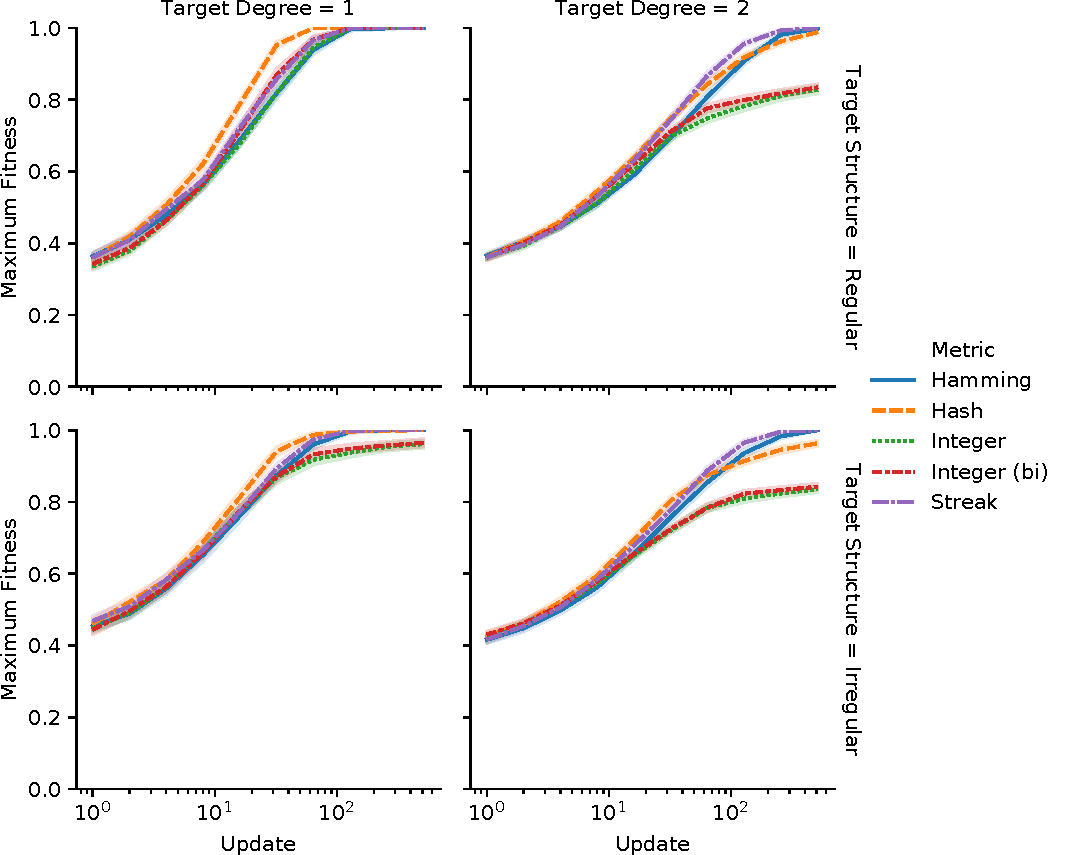
\includegraphics[width=\linewidth]{target_evolve/viz=max-fitness-line+_data_hathash_hash=673d309ab90e91d1+_script_fullcat_hash=fe3ddc711c5abfad+ext=}
\end{minipage}
\begin{minipage}{\linewidth}
\caption{
Maximum fitness by update over replicate runs for each metric's best-performing mutation rate.
Note log-scale x-axes.
Shaded area represents 95\% confidence intervals.
}
\label{fig:evolve_bests}
\end{minipage}
\end{center}
\end{minipage}

